\chapter{Architecture design} \label{ch:architecture}

\section{Architecture overview}

The whole project is divided into two main parts. The purpose of the backend is to execute the Arduino code and simulate the change on the board's pinout. The purpose of the frontend is to reflect these changes on a user defined logical circuit, while offering the user control over the simulation. We chose to implement the backend in C++ and the frontend in C\#. Both backend and frontend are running in its own separate process.

\begin{figure}[ht]
    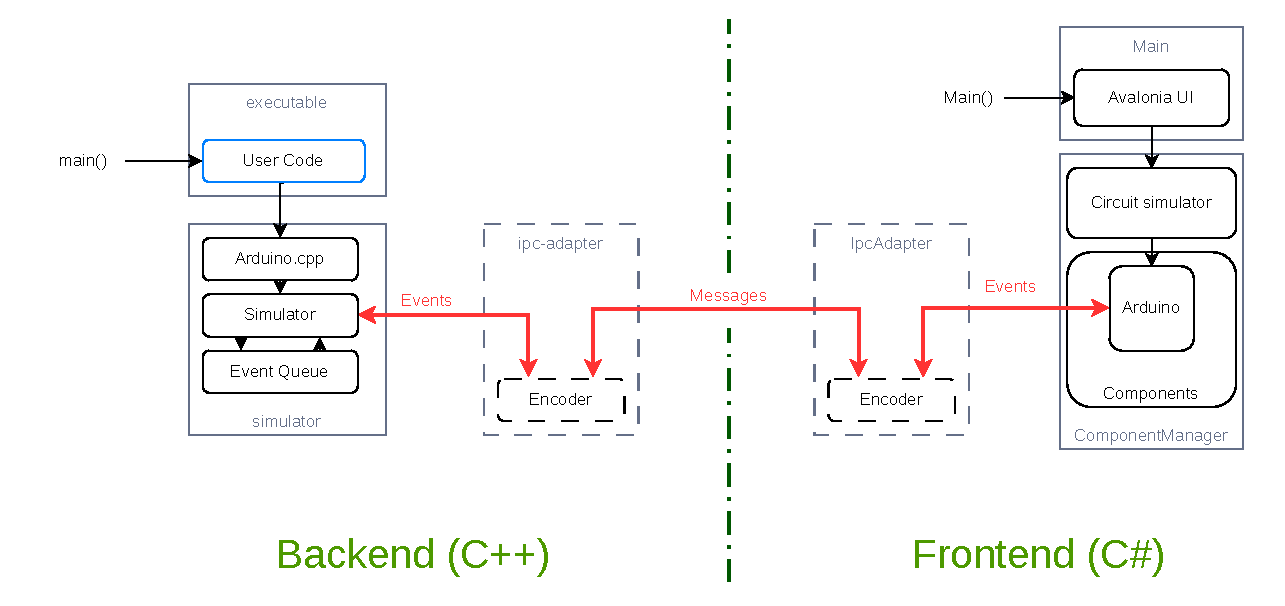
\includegraphics[width=\textwidth, keepaspectratio]{img/overall-architecture.pdf}
    \caption{Top-level architecture overview}
    \label{fig:architecture}
\end{figure}

The Figure \ref{fig:architecture} shows the most important systems in each process. The user code is compiled together with the \texttt{executable} module of the backend. The declarations in the header \texttt{Arduino.h} prepended to the top of the \texttt{.ino} is implemented by a mock library \texttt{Arduino.cpp}. For each observable action an event is created and passed to the singleton \texttt{Simulator} class to compute and put into an event queue. The event is also communicated to the frontend process.

In the frontend the events are consumed by the \texttt{Arduino} component, one of several components predefined as part of the \texttt{ComponentManager} project. This project is responsible for loading user-defined components and scenes, which connect the components together in a circuit. The circuit is simulated in the same project. The user interface is implemented in the \texttt{Main} project using Avalonia UI as a framework. Interacting with the UI may invoke new events in the \texttt{Arduino} component. Those are sent back to the backend's event queue in the same manner as they were received.

The IPC Adapter is an interface implemented in each process responsible for encoding and decoding the events into a standardised format and relaying to the other process.

\section{Inter-process communication}

Implementing processes that depend on each other comes with certain challenges. Processes always run concurrently, so a variety of synchronization techniques must be applied to avoid race conditions. Before that we need to determine how will the processes exchange data. Process is a kernel level mechanism, thus approaches to handle the exchange can vary between operating systems. These mechanisms are what is called \textit{Inter-process communication}, or IPC for short.

\subsection{Considerations}
There is a technical and an engineering reason for splitting the work into more than one process.

The user must be able to have full control over the frontend user interface at all times, even while the Arduino code is being debugged. Every common debugger blocks all running threads of a process, when a breakpoint is hit. \xxx{elaborate} If the GUI has been part of the same process as the systems running the simulation, it would freeze and become unresponsive every time a breakpoint is hit. The only way to avoid this behavior is to separate the GUI to a different process. We want to support breakpoints in our project, as they are the most useful tool in a debugger's toolkit.

Splitting the application into multiple processes is actually a common practice among larger pieces of software. The program of each process can be written in a different programming language and thus delegated into teams with different competencies. They mark clear separation of concerns and force a solid interface design. Each process is easily swappable for another implementation with the same interface while the other processes are still running. In our case, the GUI process could be replaced by a web client, a CLI client, or an IDE add-on.

There are more than a few ways to handle IPC on every OS. The ones that we implemented are \textit{TCP stream} and \textit{shared memory}. These are among the most common approaches available both on Windows and Linux. In either case, we must clearly define what the shared data represent. Although shared memory has more flexibility than TCP, we stuck to sending discrete text or binary messages of predetermined format over time, to keep the implementation simpler and the two approaches interchangable.

Another question is what will we encode in our message. At first we encoded the full state of the simulated Arduino in \textit{snapshots} but due to its various shortcomings we later switched to sending discrete \textit{events}. So the simulator in the backend and its interpratation in the frontend both operate in terms of events, but TCP and shared memory modules only understand the notion of sending and receiving messages with very distinct interfaces. That's why we need to design an adapter in both processes and for both IPC methods that sets up the mechanism and encodes or decodes the passing messages into structured event data the simulation logic understands. The IPC adapter then informs the other systems in it's process any time a new event is received.

\subsection{Snapshotting}

In the early iterations, a snapshot of the Arduino state was sent over one message. That included the pinout state, pin modes, timer, etc. The state was periodically requested by the client with a \textit{Read} message without payload. When a new value is read on an input pin in the frontend, a \textit{Write} message with the state as payload would be sent to the server and the values of input pins would be overwritten atomically to the backend's internal state. 

This approach was easy to implement but flawed. The main issue was the frequency of reads. At lower frequencies, the system is prone to temporal aliasing. \xxx{Find temporal aliasing definition}. Some events, like very short impulses, can be missed completely. This is not much of an issue in purely combinational circuits. But we want our frontend to support stateful components, e.g. shift registers present on the Funshield, which are controlled by digital writes less than a microsecond a part.

Highering the frequency to such an extent is not viable. \xxx{elaborate}

\subsection{Events}\label{subsec:events}

Right now synchronization between processes is maintained by recording every significant event produced by either the backend or the frontend, and sending it to the other process. Each process is equipped with an event queue, that consumes the events in order of the least recent to the most recent. Consuming an event means invoking the appropriate function based on the type of the event with arguments stored in the event's signature. 

The Arduino object in the frontend has no logic on its own, so the only consumed events are those produced by the backend. For that reason a simple queue is sufficient, and no further synchronization is necessary. In the backend however, both simulator's and frontend's events are consumed. Sending an event to the frontend and receiving direct consequeunces of the event back can involve a significant time overhead. In the meantime the simulator produces more events that are consumed almost instantaneously. We need to ensure that the events are consumed in a valid order. We also need a robust queue implementation that isn't prone to race conditions.

An event is labeled with two timestamps. Timestamps don't have to be based on a real clock, the only requirement is that it is a non-decreasing sequence of numbers. The first timestamp sent is the simulation time, the time as perceived by the Arduino being simulated. That is time given by a clock that is started right before the \texttt{setup()} is invoked. It can be manipulated by the user by pausing or slowing down. This is to aid the user while analyzing the logs of the simulator.

The other timestamp included is \textit{Local virtual time} (LVT)\footnotemark. Each process holds its own integer value of LVT. This number is increased with newly produced events and events received from the other process. When a decision has to be made on which event to consume next (like in the case of the backend's queue), the event with lower LVT is chosen. The relation $LVT_{1} > LVT_{2}$ means that the event with $LVT_{1}$ happens after the event with $LVT_{2}$. In other words, event 1 is the consequence of the event 2 regardless of the real time passed between the events.

The rest of the information stored in an event is its type and arguments. The type corresponds to the action taken after the event is consumed, like writing to a pin or changing pin mode. Each type can define up to 3 integer parameters, e.g for a \textit{write} event that is id of the pin, and a digital value we want to write to it. By limiting the number of arguments, we intend to avoid heap allocation of these events, which could considerably slow down the simulation with programs that produce a lot of events in a short time.

There are many ways to encode such an event into a message. Currently the only encoder implemented in this work is the text encoder, which parses values of events into human readable strings separated by a colon. The messages themselves are separated by a semicolon. This particular encoding is quite space ineffective, but it helps a lot during debugging of the IPC systems.

\footnotetext{The terminology and principles are inspired by the \textit{Optimistic synchronization} paradigm in distributed systems. In this paradigm, the events are consumed as fast as possible, and then rolled back once an event with a lower LVT than the ones consumed appears (so called \textit{Time Warp} mechanism). But Time Warp is not viable for simulating code of a high level language like C++ without custom memory management, and in our implementation it isn't even necessary. \cite{fujimoto_parallel_2001}}

\subsection{TCP stream}

Messages can be sent and received through a stream of data on a TCP connection. TCP is commonly used to send data over a network, meaning backend and frontend processes can run on different machines. But listening to a connection on the same machine on the same port works just as well. TCP messages are guaranteed to arrive in the same order as they were sent.

The backend implements the TCP server, while the frontend implements the client. The implementations and design considerations behind these are very different based on the language they were written. But in both cases TCP handlers need to run on their own threads, due to how heavyweight \xxx{elaborate} they are. There is a buffer to which read bytes are stored from an OS network stream. These are passed as a chunk to a higher level message handler that splits the chunk into individual messages according to predetermined delimeter character. When a message needs to be sent from another thread, it is passed to the message handler where it is posted to the end of a queue and is scheduled to be processed by the OS.

There is a minor limitation of IPC over TCP that makes the debugging experience of the user's code uncomfortable. As we established, hitting a breakpoint will block all running threads of the process, including the thread with the TCP handler. When stepping through the lines of the code where events are produced, the TCP thread has to schedule posting of the message with the event, and it takes time for it to be eventually sent. In many cases the TCP thread won't be fast enough to send the message in the time the main thread progresses to the next line where a breakpoint will be hit again. As a result, consequences of the event won't be reflected in the frontend process until another one or more lines have been stepped through. This is the main reason we decided to also implement IPC with memory mapping, even though TCP is fully functional.

\subsection{Shared memory}

Memory mapping is the functionality of an operating system to relate a region of main memory 1:1 to a region in the address space of a process. This is an important idea in establishing a virtual memory of a process, but OS objects can be mapped as well. It could be either a \textit{memory-mapped file}, contents of a disk file moved to the RAM. Or it could be a special OS object called \textit{shared memory}, living in the kernel heap, specifically designed for IPC. In both cases, multiple processes can map the same memory region to their own address space. Thus they have access to the same data.

The terminology and API differ significantly between Linux and Windows, but with the use of the right libraries, the differences can be abstracted away and used as a single concept. So from now on we refer to the idea of mapping the same memory region to multiple address spaces as \textit{shared memory}.

This tool is very powerful, we can address the shared data by pointers as we would with any other data of the process. There is also no need for system calls once the the memory has been mapped. No special instructions need to be used for reading or writing and all changes are immediately visible on all of the processes that map the same region. As long as we do the writes in the simulating thread, we avoid the problem with delayed observations during debugging we encountered with TCP.

In the shared memory region, we establish a data structure that stores messages in a sequential order. We opted for a circular buffer to fully utilize the limited space of the region. There are actually two non-overlapping buffers in the same region together with a few bytes of metadata about their current state. A process consumes messages from one buffer while producing new messages to another. This is to avoid numerous race conditions that would occur while writing and reading from the same buffer while keep the synchronization mechanism lock-free.

As for the metadata, for each buffer a position after the last consumed and produced message is stored. It is important to never store references as pointers in the shared memory itself. The memory region will be most likely mapped to different addresses in each process. Because of that the \textit{producer offset} and \textit{consumer offset} are regular integers denoting the distance from the first adress of the buffer in bytes. When the offsets are equal, it means the buffer is empty. We don't care about concurrent updates of these offsets, one process changes only one of the offsets for the duration of the simulation.

\begin{figure}
    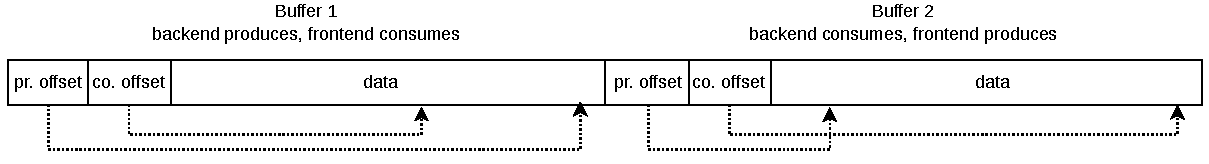
\includegraphics[width=\textwidth, keepaspectratio]{img/circular-buffer.pdf}
    \caption{Memory layout of the shared memory region}
    \label{fig:circular-buffer}
\end{figure}

\section{Backend}

\subsection{The simulation}

\begin{figure}[ht]
    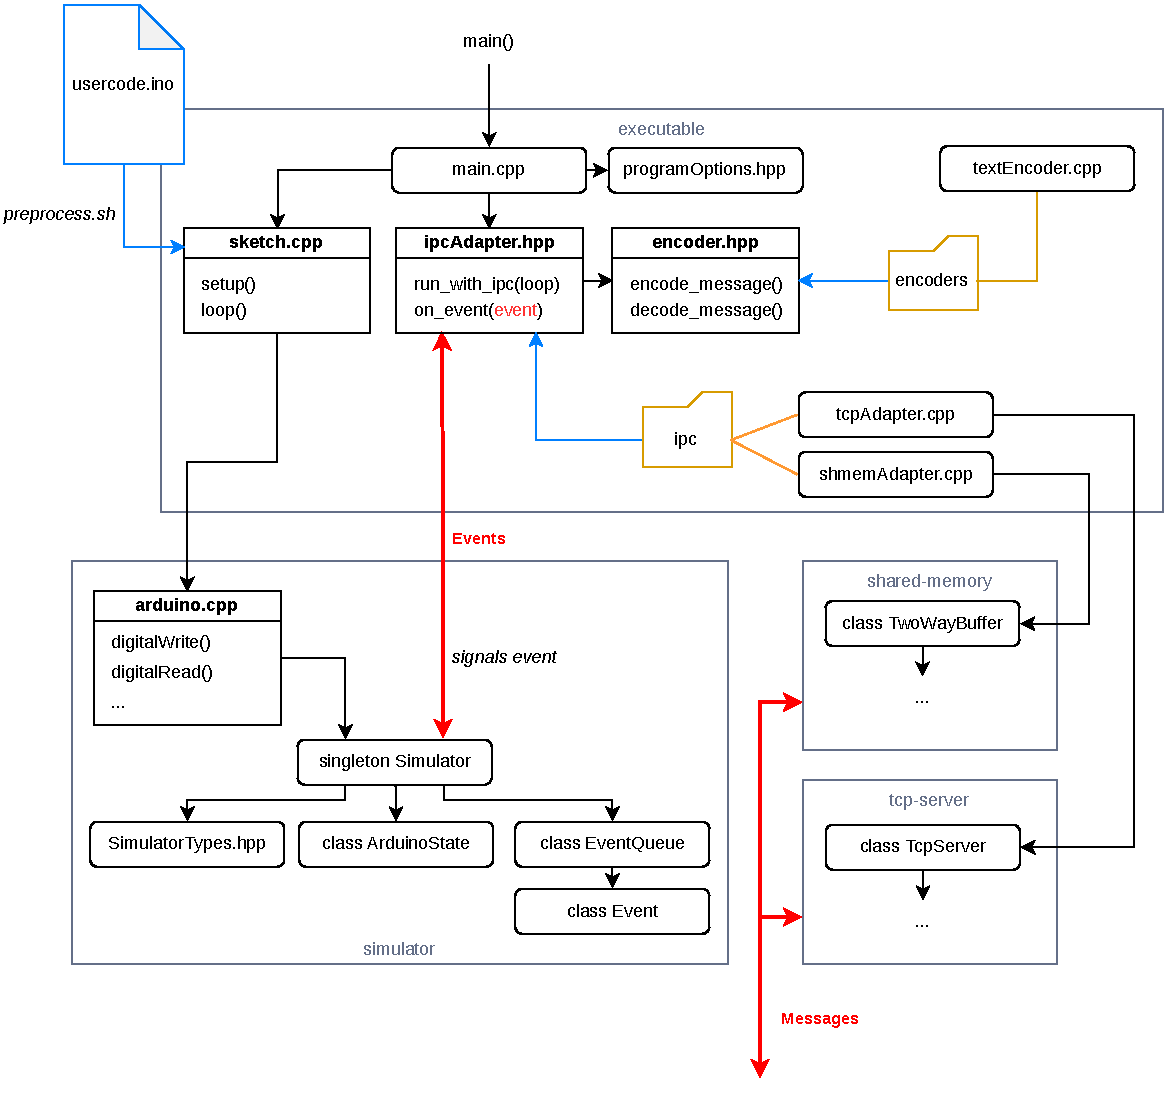
\includegraphics[width=\textwidth, keepaspectratio]{img/backend-architecture.pdf}
    \caption{Backend architecture}
    \label{fig:backend}
\end{figure}

The language choice for backend was obvious, the \texttt{.ino} file is a syntactically valid C++ code. We include the code in the project by passing it as an argument to the \texttt{preprocess.sh} script (\texttt{preprocess.bat} on Windows). Inside we use the \texttt{arduino-cli} tool with the right arguments to apply very light prerpocessing to the file, like adding function declarations to the top or including the \texttt{Arduino.h} header. Important additions are the \texttt{\#line} directives, which link to the definitions in the original \texttt{.ino} file. Thanks to these, breakpoints can be added to the \texttt{.ino} file and debugged as if the file itself was part of the project, completely with stepping through lines and inspection of variables. The file is then saved as \texttt{sketch.cpp} in the directory of the \texttt{executable} module where it is picked up by the CMake configuration and included in the \texttt{main.cpp}. The functions declared by the \texttt{Arduino.h} header file, like \texttt{digitalWrite} or \texttt{millis} are implemented in a custom mock library \texttt{Arduino.cpp} in the \texttt{simulator} module. Instead of instructing the AVR chip, as the real implementation would, the mock definitions create events and pass them to the \texttt{Simulator} for enquing and consumption. 

The \texttt{Simulator} singleton class is the beating heart of the backend. It is responsible for handling the events and the event queue, managing the Arduino state, logging changes and keeping track of time. It is initialized in \texttt{main.cpp} and used frequently throughout the \texttt{executable} and \texttt{simulator} modules. The \texttt{Simulator} holds the instance of the \texttt{ArduinoState} class, representing the digital states on its pins, current pin modes and the inner timer of the Arduino. It also holds the instance of the \texttt{EventQueue}, which stores both local and remote events waiting for consumption. The \texttt{SimulatorTypes.hpp} is a header file with very few type defintions commonly used in the \texttt{simulator} module.

\subsection{Events and IPC}\label{subsec:cpp-events}

The \texttt{Event} struct is just a "recipe" for what changes should the \texttt{Simulator} do to the \texttt{ArduinoState}. It holds a lambda function, corresponging to an event's type that is executed only after the event is put in the event queue and consumed in the order described in the section \ref{subsec:events}. The struct defines static functions that create new event instances with these predefined lambdas with the event type's parameters. When a local event is consumed, i.e. the lambda is executed, the event is signalled back to the \texttt{executable} module through a callback, that has been passed to the \texttt{Simulator} during initialization. This way the event can be sent to an IPC adapter, regardless of the used implementation, without a circular dependency on the \texttt{executable} module.

The IPC adapter itself is an interface of two functions declared in the \texttt{ipcAdapter.hpp}. \texttt{run\_simulator\_with\_ipc} initializes the IPC mechanism. It takes the simulator loop function as an argument and executes it after IPC has been set up. That is because the IPC usually needs to create new threads that cannot be joined before the loop stops running. The loop function itself is defined in \texttt{main.cpp} and it contains both the \texttt{setup()} and \texttt{loop()} calls from the user's code.

The \texttt{on\_event} function of the adapter is the callback passed to the \texttt{Simulator}. It encodes the event into a message and sends over IPC to the remote process. Listening to events of the remote process occurs on a different thread than the one with the simulator loop. Incoming messages are decoded into \texttt{Event} structs and sent directly to the event queue in the \texttt{Simulator}. \texttt{encode\_message} and \texttt{decode\_message} are functions declared in yet another interface in the \texttt{encoder.hpp} header. It's implementations are in the \texttt{encoders} directory, i.e. only \texttt{textEncoder.cpp} at the moment.

Implementations of the IPC adapter are located in the \texttt{ipc} directory. The \texttt{tcpAdapter.cpp} depends on the \texttt{tcp-server} module, while the \texttt{shmemAdatper.cpp} depends on the \texttt{shared-memory} module. Which one is used depends on the chosen compilation target. The \texttt{tcp-server} module contains definition of the TCP server and mechanisms for accepting new connections and handling the stream of data using the \texttt{boost::asio} library. The \texttt{shared-memory} module contains memory mapping mechanisms using the \texttt{boost::interprocess}, implementation of the circular buffer and the producer-consumer pattern using two buffers.

\subsection{Utilities}

\subsubsection{Logger} \label{subsub:logger}

There are additional utility modules not shown in the figure \ref{fig:backend}. One of them is the humble \texttt{logger} used extensively throughout the project. The \texttt{ILogger} abstract class exposes the \texttt{log} function accepting either a raw string or an \texttt{IMessage} abstract struct. Structs inheriting form \texttt{IMessage} represent unified formatting of a message with a timestamp and a level of verbosity. The verbosity levels from the highest to lowest are \textit{Debug}, \textit{Info}, \textit{Warning} and \textit{Error}. The messages of higher verbosity levels can be ommitted from the logs by setting the appropriate command line option. \texttt{ILogger} offers shorthand functions for logging these general messages, but more specific ones can be defined as well.

The module comes with \texttt{FileLogger} implementation of the \texttt{ILogger}. It creates or opens a file and dumps the logs inside. To avoid race conditions while writing to the files, two of these loggers are used in the project. One is owned and used by the \texttt{Simulator} singleton for logging inner workings of the Arduino. The other is owned by the IPC adapter and used for logging the exchanged messages or potential failures of the IPC mechanisms.

\subsubsection{Timer}

The other utility model is \texttt{Timer}. It is used to track time from the start of the simulation. The simulator holds two of these timers, one for \textit{real time} and one for \textit{simulation time}. Although there is no difference between them right now, the intention is to apply effects like stopping or slowing down to the simulation time timer from the frontend, so that functions like \texttt{millis} work consistently with disturbances caused by the frontend. Functions returning real time and simulation time are passed to the file logger as a source of its timestamps.

\section{Frontend}

\subsection{The presentation}

\begin{figure}
    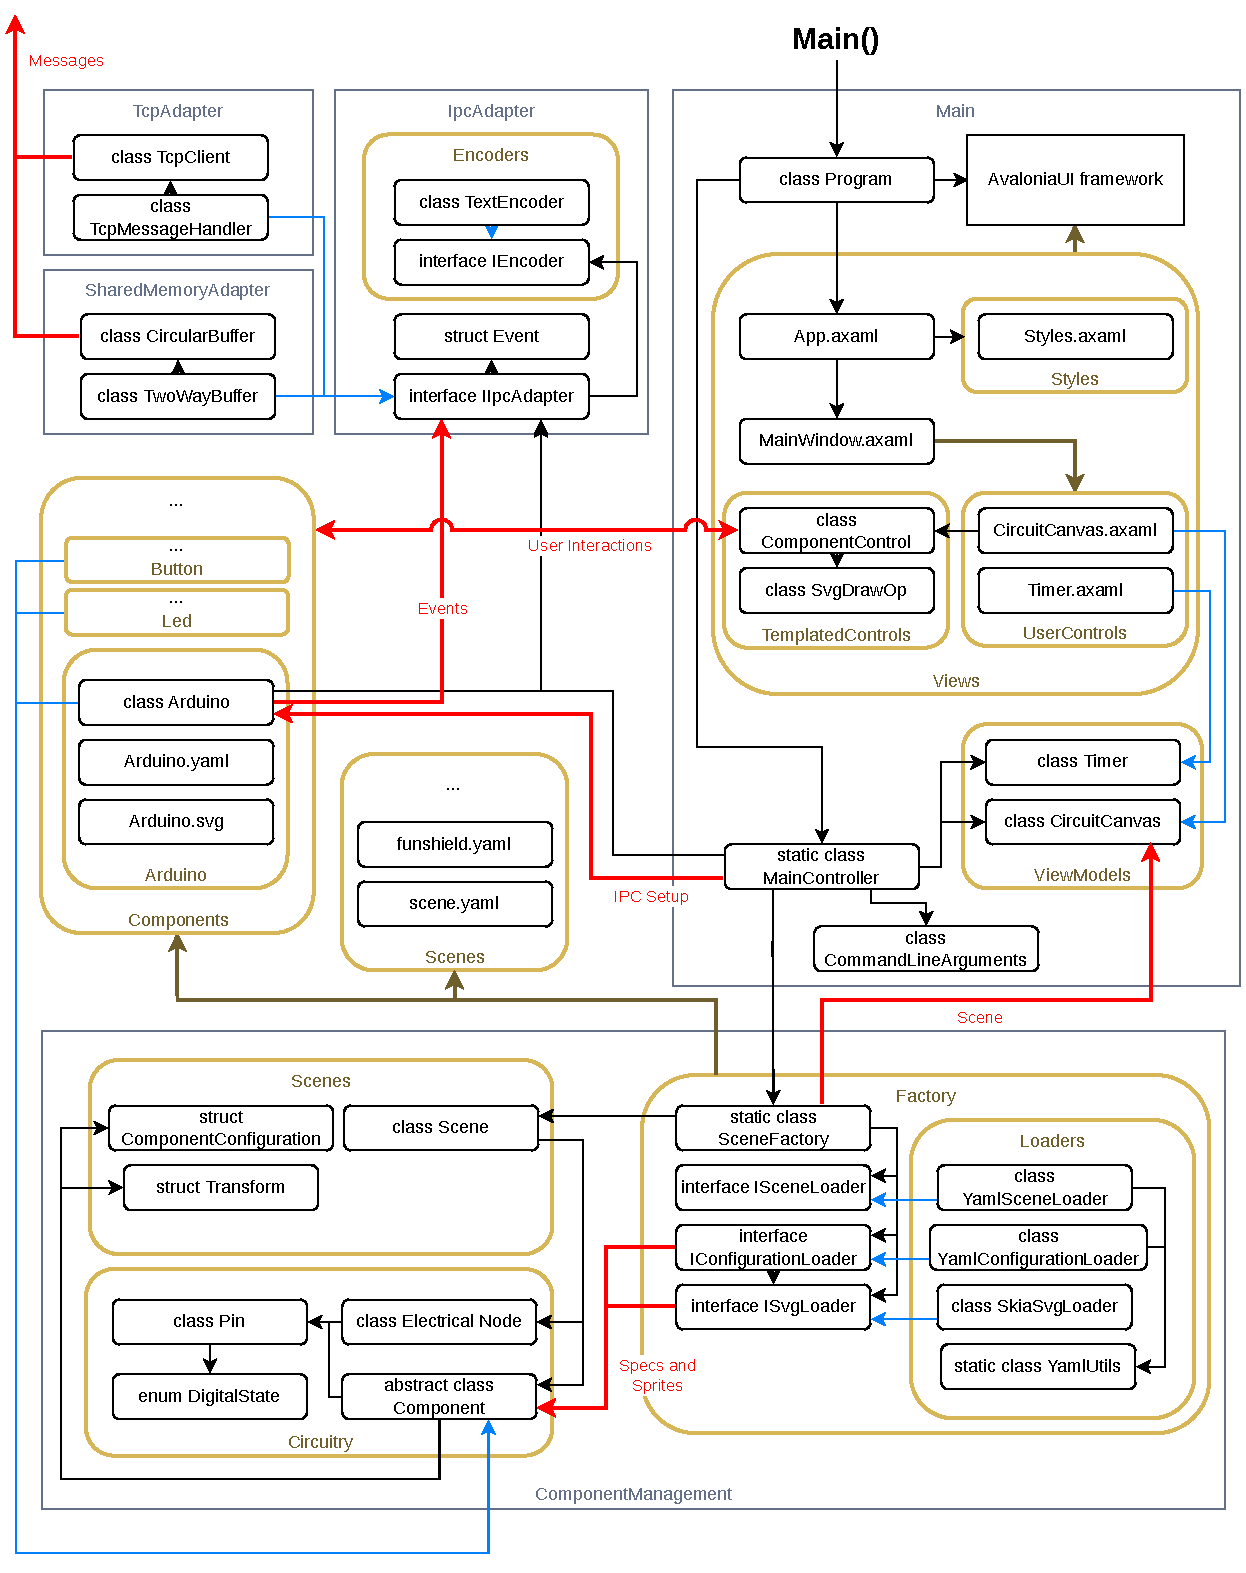
\includegraphics[width=\textwidth, keepaspectratio]{img/frontend-architecture.pdf}
    \caption{Frontend architecture}
    \label{fig:frontend}
\end{figure}

The frontend is written in C\#. We consider the language to be more convenient for writing many of the essential systems than its C++ counterpart. That includes handling the graphics, the user interactions and parsing numerous configuration files needed for extensibility of the application. Libraries are also much easier to set up and compile thanks to NuGet.

For the GUI we decided to use Avalonia UI. Avalonia is a popular open-source cross-platform .NET framework, used by major companies like JetBrains or Unity. It is based on the Microsoft's WPF framework utilising the same XAML markup language and many of the same core principles. We chose it exactly because neither WPF or its cross-platform successor MAUI are available on Linux, one of our target platforms. We only include Avalonia in the Main project of the frontend, as this is the only project responsible for rendering.

Our humble GUI consists mostly of the circuit canvas. A zoomable and pannable space where the \textit{components} of a circuit can be placed to specific coordinates, uncostrained by the usual layout structures of Avalonia. Arrangement of these components is called a \textit{scene}. Each of the component types have its own set of SVG images that are drawn to the canvas. We refer to them as \textit{sprites}. Each individual component always references one of its sprites, conveying the current state to the user. A sprite on the canvas can be clicked on (e.g. a button) to generate some kind of response. Of course, these features are not built into Avalonia, so we need to create custom Avalonia \textit{controls} to achieve them.

\subsubsection{Model-View-ViewModel}

The preferred architecture for Avalonia applications is \textit{MVVM}, or \textit{Model-View-ViewModel}. \textit{View} is the visual layout of the window and its parts. It is written in \textit{XAML} (Extensible Application Markup Language) in files with the \texttt{.axaml} extension. In Avalonia's case, elements of a view are called \textit{controls}. Those can be buttons, labels, containers, etc. 3 types of custom controls can be created in total, our frontend utilizes \textit{user controls} and \textit{custom-drawn controls}. User controls are themselves views built up in XAML from other controls. This is perfect for our \texttt{CircuitCanvas} view, as it is just a list of component controls enveloped in a built-in \texttt{Canvas} panel. The custom-drawn controls are defined as C\# classes, inheriting from the \texttt{Control} class, and defining it's own rendering logic by overriding the \texttt{Render} method \cite{avalonia_custom_controls}.

We need to implement the visuals of our components using custom-drawn controls, as there are no built-in or library controls that can draw a precompiled SVG image and swap it during runtime. Thus we define a \texttt{ComponentControl}, that calls a custom drawing operation in its \texttt{Render} method. That is defined by the \texttt{SvgDrawOp} class, which takes a sprite and a transformation matrix as arguments, applies visual transformations on the image and instructs the Avalonia's rendering pipeline to show it in the parent view.

XAML views bind to data and events in a \textit{viewmodel}, which manipulates with data shown in the view. A model then is the raw data passed to the viewmodel, accessed by some database or a service, or produced by the business logic. View is aware of the viewmodel and viewmodel is aware of the model, but not vice versa. In ideal case, the model should be agnostic about the UI technology used. \cite{avalonia-mvvm}

Our model is the abstract \texttt{Component} class implemented by various types of components, like LEDs, buttons or our Arduino. A list of the \texttt{Component} instances is stored in \texttt{CircuitCanvas} viewmodel, and each instance is passed to a \texttt{ComponentControl} in the \texttt{CircuitCanvas} view. This and all other initialization steps of the application are orchestrated by the static \texttt{MainController} class.

\begin{figure}
    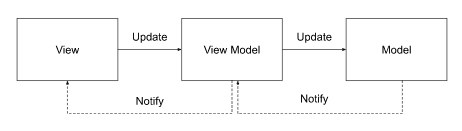
\includegraphics[width=\textwidth, keepaspectratio]{img/mvvm.png}
    \caption{MVVM architecture {\cite{avalonia-mvvm}}}
    \label{fig:mvvm}
\end{figure}

\subsection{The logic}

Only a minor part of the frontend is actually written with Avalonia. The business logic of the aforemention \texttt{Component} model is all encompassed in the \texttt{ComponentManagement} project. That means parsing of the components definition, creating instances of a scene, and the simulation of the circuit. This project is completely unaware, that it will be rendered with Avalonia specifically.

The circuit can be thought of as an unoriented multigraph, where the nodes of the graph are both \textit{electrical nodes} and the \textit{components}. All neighbors of an electrical node are components, and all neighbors of a component are electrical nodes. An edge of the graph represents a conductive connection between an electrical node and a \textit{pin} of a component. Components usually have multiple pins. 

In a digital circuit, an electrical node always obtains one of two digital states, \textit{high} or \textit{low}, which is given by states of pins it is connected to. When a high state is written into a pin, we say it is \textit{driving}. When a low state is written into a pin, it becomes not driving again. The digital state of an electrical node is high precisely when at least one of the pins it is connected to is driving. A change in the state of an electrical node is propagated through all of the connected pins. Components can react to this change by writing new states to their other pins creating a chain reaction of state changes in the circuit.

\subsubsection{Components}

The frontend's user is encouraged to extend the simulation with their own implementations of the abstract \texttt{Component} class. That is done by creating a new \textit{component directory} with the name of the component. The shared path to all component diretories is specified as one of the command line options of the frontend. The static information about the component type is stored as a record \texttt{ComponentConfiguration}, created from the files in the directory. The required files are a YAML file with metadata and at least one SVG file for the sprite. The YAML file contains in the very least a name to identify the component type, and a list of the component's pins. The pins can be defined either as an enumeration of their names, or as a single integer, that represents the total count of unnamed pins identified by their index.

The \texttt{Component} base class provides multiple virtual methods with the \texttt{On*} prefix. These are called upon changes in the circuit or as a result of a user interaction. The most important one is the \texttt{OnPinStateChanged} with the \texttt{Pin} object passed as an argument. This is the primary way of defining the component's logic. \texttt{OnControlPress} and \texttt{OnControlRelease} are other useful methods for interactible components, such as buttons. The base method \texttt{UpdateSprite} changes the rendered sprite to a different one, identified by the name of its SVG file. The base \texttt{GetPin} method returns a \texttt{Pin} object of the component's instance identified either by its name or index. Digital states are read and written through this object. 

Usually, specific pins have inherent semantics of being used only for reading or only for writing. This property can be set explicitly on the \texttt{Pin} object with \texttt{MakeReadOnly} and \texttt{MakeWriteOnly} methods. Read only pins refuse write attempts from the component's logic and write only pins refuse notifying a component with a new state from node's propagation. General pins, defined by method \texttt{MakeGeneral} don't have these constraints. Incorrect use of pins with these semantics is followed by a warning in the simulation logs.

\lstinputlisting[language=yaml, caption={Component configuration example: Led.yaml}]{../frontend/ComponentManagement/Components/Led/Led.yaml}

\subsubsection{Scenes}

The final form of the graph is achieved with creation of the scene. The YAML file of the scene consists of two sections. In the \texttt{Components} section, individual instances of \texttt{Component} subtypes are defined. They must have a unique name, and they should specify a graphic transformation, i.e. position, rotation and scale. This triplet of 2D vectors is composed into a \texttt{Transform} struct and passed into the \texttt{SvgDrawOp} as a transformation matrix. The \texttt{Nodes} section defines individual electrical nodes. A single node in this file is represented as a list of component-pin pairs, where the components are identified by their instance name in the \texttt{Components} section, and the pin is identified by its definition in the \texttt{ComponentConfiguration} of the given \texttt{Component} subtype.

The creation of the scene is comprised of a series of parsers in the \texttt{Factory} directory. There is an interface for each of the file types, i.e. the scene, component configurations and SVG files. Each has exactly one implementation in the \texttt{Loaders} directory, using \texttt{YamlDotNet} and \texttt{SvgSkia} libraries. They are put together in the static \texttt{SceneFactory} class, where component subtypes and instances are finalized. The results is a complete \texttt{Scene} object with initialized \texttt{Component} instances and \texttt{ElectricalNode} lists. The \texttt{SceneFactory} is called by the \texttt{MainController} in the \texttt{Main} project, which passes the scene to the \texttt{CircuitCanvas} viewmodel.

\lstinputlisting[language=yaml, caption={Scene example: minimal.yaml}, label={lst:scene}]{../frontend/Scenes/minimal.yaml}

The example scene in the listing \ref{lst:scene} contains 2 LEDs, 1 button and 1 source of voltage. Source, which has one pin that is always driving, is connected to the 0th pin of the button, which reads a high value of the node. Both LEDs are connected to the 1st pin of the same button. Pressing the button will copy the digital state from pin 0 to pin 1, and thus lights up the LEDs.

\subsection{The Arduino component and IPC}

Arduino is one of the component subtypes of the \texttt{ComponentManagement} project. It is a partial class divided into 2 files. In \texttt{Arduino.cs} it overrides virtual methods and deals with interaction with the circuit. In \texttt{Arduino.Events.cs} it creates events and sends to IPC. It also calls its own method from \texttt{Arduino.cs} when a new event arrives, based on its type and arguments. The adapter is now defined as an \texttt{IIpcAdapter} interface, which is owned by the Arduino component. Events are exchanged through this interface.

The interface is defined in the \texttt{IpcAdapter}, and is implemented by the \texttt{TcpAdapter} and \texttt{SharedMemoryAdapter} projects. It declares methods for connecting to IPC and sending messages. It also declares a C\# event called \texttt{ReceivedEventEvent}, which is invoked after decoding a message incoming from the backend, with the decoded \texttt{Event} struct as an argument. The Arduino component is subscribed to \texttt{ReceivedEventEvent}.

The \texttt{IpcAdapter} project also contains message encoders and a definition of the \texttt{Event} struct. The C++ and the C\# version of the \texttt{Event} struct have the same signature, with the exception of owning a lambda function (described in \ref{subsec:cpp-events}). The lambda is not necessary for the frontend, as there will be only one source of events executed in the frontend, the ones received by the backend. They don't have to be put in a queue, they can be consumed immediately as they come. Frontend also produces events, e.g. when value on an Arduino's input pin is changed from the circuit, but those are never consumed by the frontend. It is the reponsibility of the backend to handle them.

\texttt{IEncoder} and its \texttt{TextEncoder} implementation are analogous to \texttt{encoder.hpp} and \texttt{textEncoder.cpp} in the backend. The interface declares \texttt{EncodeEvent} and \texttt{TryDecodeEvent}, which transcribe events structs into human-readable strings and vice versa.

\subsection{Utilities}

\subsubsection{Logger}

The \texttt{Logger} project is analogous to its backend counterpart (\ref{subsub:logger}). It provides logging to a file with 4 levels of verbosity, that can be set up with a command line argument. Two loggers are used in the frontend as well, one for IPC and one for circuitry logs. There is one additional implemenation of the \texttt{ILogger} called \texttt{CompositeLogger}, which holds list of loggers, and logs into all of them simultaneously. This mechanism anticipates a need for another logger implementation, which will display the log messages in the GUI using Avalonia.